\chapter{Donaldson-Witten theory in MQ formalism}
\label{chapter4}
% See AJ intro
In finite dimensions, the Mathai-Quillen formula gives an explicit differential
form representative of the Euler class. 
It was shown by Atiyah and
Jeffrey \cite{atiyahlagrangians} that not only can the zero dimensional
Donaldson invariant can be identified with the Euler number of a vector bundle
over $\mathcal{A} /\mathcal{G}$, but the Donaldson invariants in general can be
written as an integral of a Mathai-Quillen type form over the gauge equivalence
classes of irreducible connections, similar to (reference Gauss-Bonnet formula
with Mathai-Quillen).
Moreover, they have been able to reproduce Witten's
action functional from twisted SUSY YM theory term by term from purely geometric
considerations.

Conversely,
the Mathai-Quillen formalism makes it possible to construct a cohomological field
theory starting from a moduli problem.

\section{Thom form analog for principal bundles}
Before we construct the Atiyah-Jeffrey formula, we first need to develop an
analog of the Thom form for a principal $G$-bundle $P\to M$. Assume $G$ is
a connected compact Lie group with $\dim G = d, \dim M = n$. 
We wish to construct a differential form  $W\in \Omega^d(P)$
such that its integral along the fiber equals 1, so that by 
Proposition \ref{prop:projection_formula}, for all $\beta\in \Omega_c^B(M)$
\begin{equation} \label{eq:principal_thom_local}
	\int_M \beta = \int_P \pi^*\beta \wedge W
\end{equation}
Of course, we will need an orientation on $M,G$ and $P$.    
%local product orientation on $P$ (see \cite[p.64]{bott_tu}).   

\begin{figure}[htb]
	\hfill
	\begin{minipage}[c]{0.61\textwidth}
		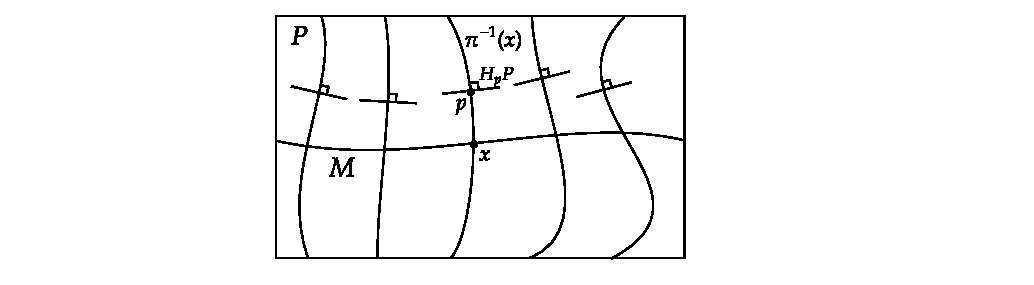
\includegraphics[trim={45mm 4mm 5cm 2mm},clip,width=\textwidth]{figs/connection_from_metric.pdf}
	\end{minipage} 
	\begin{minipage}[c]{0.38\textwidth}
        \caption{Horizontal subspaces defined by orthogonal complement}
        \label{fig:connection_from_metric}
	\end{minipage} 
\end{figure}
Denote by $\omega \in \Omega^1(P,\g)$ the connection on
$P$ induced by the metric on $P$ so that the horizontal and
vertical subspaces are orthogonal complements. Let $\eta_1,\ldots,\eta_d$ be an 
orthonormal basis for $\g$ consistent with the orientation on $G$.
We will show that
\begin{equation} \label{eq:principal_thom}
W := \int^B \exp(\omega) d\eta 
= \int^B \exp(\omega_a\eta_a) d\eta = \omega_1 \wedge \cdots \wedge\omega_d
\;\in \Omega^d(P)
\end{equation}
is the desired vertical volume form. Multiplication inside the Berezin
integral occurs in the graded tensor product $\Omega(P)\otimes \g$, 
so $\omega_a\eta_a$ all have degree two.

The integral along the $G$-orbit 
$\pi_*:\Omega^{*}(P\times V) \to \Omega^{*-d}(P\times_G V)$ is defined as in 
section \ref{section:fiber_integration}, where the integral defined by 
pulling back to a form on $G$ via a trivialisation
$\psi:G\xrightarrow{\simeq} \pi^{-1}(x)$.   

% construct left invariant metric on $G$ first
We will now turn $G$ into Riemannian manifold by 
extending a metric on $\g$ to $T_gG$ via left translations. That is, define
$\gen{u,v}_g = \gen[*]{DL_g^{-1}(u),DL_g^{-1}(v)}_e$ where $u,v\in T_gG,L_g(h) = gh$.
By construction, this is a left-invariant metric. In fact, because $G$ is
connected and compact we can turn it into a
bi-invariant metric by Haar integrating the metric: $\gen{u,v}:=\int_G
\gen{DR_gu,DR_g v}$.

\begin{prop}
	For all $p\in P$,  $L_p^* W \in \Omega^d(G)$ is equal to the unique
	Riemannian volume form induced by the bi-invariant metric on $G$. 
\end{prop}
\begin{proof}
	Let $\epsilon_1,\ldots,\epsilon_d\in T^*_eG$ be the orthonormal coframe dual
	to $\eta_1,\ldots,\eta_d$. At a point $g\in G$, the tangent vectors are
	transported to  $DL_g \eta_i$ while the coframe is transported to 
	$\epsilon_i\circ DL_{g}^{-1} \in T^*_gG$, where $L_g$ is left multiplication
	by  $g$. Then the unique Riemannian volume form is given by
	\[
	    \epsilon_1\circ DL_{g}^{-1} \wedge \cdots\wedge \epsilon_d\circ DL_{g}^{-1}
	\] 
	The covectors are orthonormal in the induced metric on $T^*G$ because the 
	metric is left invariant. For $X\in \g$, the pullback
	by $L_p : G \to P_{\pi(p)}$ of $\theta := \omega_a \in \Omega^1(P)$ is
	\begin{align*}
		(L_p^*\theta)_g(DL_g X) 
		&= \theta_{p\cdot g}(DL_p \circ DL_g(X)) \\
		&= \theta_{p\cdot g}(DL_{p\cdot g} (X)) \\
		&= \theta_{p\cdot g}\paren{\odv{}{t}_{t=0} (p\cdot g \exp(tX))} \\
		&= \epsilon_a(X)
		= (\epsilon_a DL_g^{-1})DL_g(X)
	\end{align*}
	where the second and third lines are applications of the chain rule, and the
	last line uses the property $\omega(\underline{X}) = X$ of a
	connection 1-form.
	This shows that $L_p^*\omega_a = \epsilon_a\circ DL_g^{-1}$, so 
	\[
	L_p^* (\omega_1\wedge \cdots\omega_d)
	= \epsilon_1\circ DL_{g}^{-1} \wedge \cdots\wedge \epsilon_d\circ DL_{g}^{-1}
	\] 
	as required.
\end{proof}
Assume that the metric on $G$ is normalised so that the volume of $G$ is 1.
In turn, we can show that the integral along the $G$-orbit $\pi_*W = 1$. 
\begin{cor}
	The integral along the fiber of $W$ is  $\pi_*W = 1 \in \Omega^0(G)$
\end{cor}
\begin{proof}
	For $b\in M$, by definition we have $\pi_*W = \int_{\pi^{-1}(b)} W$ which is
	is computed by pulling back $W$ by a 
	local trivialisation $\psi : G \to \pi^{-1}(b)$. 
	Let $p=\psi(e)$, then $\psi(g) = \psi(e)\cdot g = p\cdot g = L_p(g)$ because
	$\psi$ is a  $G$ equivariant map. Then by the previous proposition, the
	pullback form $L_p^*W$ equals same volume form on $G$ at every point in the 
	fiber. Therefore, $\pi_*W = 1$ is the constant function on  $G$.
\end{proof}

\begin{prop} \label{prop:integral_horizontal_proj}
	Suppose $\eta \in \Omega^k(P)$ is an invariant differential form, then
	 $\pi_*(\eta \wedge W) \in \Omega^k(M)$ is the horizontal projection of 
	 $\eta$ onto $M$.
\end{prop}
\begin{proof}
	Let $b\in M, p\in \pi^{-1}(b)$. 
	We know  $W$ is a top form on the vertical tangent space, 
	since  $\omega_a$ are all linearly independent in $V_p^*P$. Let
	$dx_1,\ldots,dx_n \in H_p^*P$ be an orthonormal basis for the horizontal
	cotangent space. 

	We may assume $\eta$ is a product of 1-forms. If $\eta$ contains any factor of
	$\omega_a$, then its evaluation on all horizontal vectors will be zero, which
	agrees with $\pi_*(\eta\wedge W) = 0$. Now suppose $\eta = dx_I$, for 
	an ordered multi-index $I\subset\{1,\ldots,n\}$.
	By definition of the fiber integral, for $v_1,\ldots,v_k \in T_bM$
	\begin{align*}
		\pi_*(\eta\wedge W)_b(v_1,\ldots,v_k) 
		= \int_{\pi^{-1}(b)} (\eta\wedge W)(\widetilde{v}_1,\ldots,\widetilde{v}_k,-)
	\end{align*}
	where $\widetilde{v}_i \in TP$ is any lift of $v_i$. In particular, at a
	point $p\in \pi^{-1}(b)$, we can choose them to be horizontal lifts, then
	extend to the whole fiber by right translation $R_g$. Note that if  $v\in H_pP$, is
	horizontal, then  $DR_g(v) \in H_{p\cdot g}P$ is still horizontal because 
	the connection form $\omega$ satisfies  $\Ad_g R_g^* \omega = \omega$. 
	\begin{align*}
		\pi_*(\eta\wedge W)_b(v_1,\ldots,v_k) 
		&= \int_{\pi^{-1}(b)} \eta(\widetilde{v}_1,\ldots,\widetilde{v}_k)\wedge W \\
		&= \eta_p(\widetilde{v}_1,\ldots,\widetilde{v}_k)\int_{\pi^{-1}(b)} W \\
		&= \eta_p(\widetilde{v}_1,\ldots,\widetilde{v}_k) 
	\end{align*}
	the second line follows from $\eta$ being an invariant form: 
	$R_g^*\eta = \eta$ and that is how we've chosen the lifted horizontal
	vectors. 
\end{proof}


\section{Atiyah-Jeffrey formula}
This section is a much more thorough explanation of section 2 of the paper by
\citet{atiyahlagrangians}, where a formula for the Euler number is obtained
starting from the Mathai-Quillen Thom form. 
The purpose is to formally apply it to the Donaldson-Witten context in the next
section. We consider the following setup: 
\begin{itemize}
	\item $G$ is a compact connected Lie group of dimension $d$
	\item $P\to M$ is a principal $G$-bundle  of dimension  $2m+d$.
	\item Choose an $\Ad$-invariant metric on $\g$ using Theorem 
		\ref{thm:lie_inner_product}
	\item Similarly, construct a metric on $P$ which is invariant under the 
		action of  $G$, by averaging any Riemannian metric on $P$ with respect 
		to a Haar measure  
	\item At each point $p\in P$, this Riemannian metric defines an orthogonal
complement to the vertical tangent space. Since these subspaces are invariant
under the action of $G$, this determines a connection  $\omega$ on  $P$.
Moving forward, we will solely use this connection.
	\item $V$ is a real vector space, with $\dim V = 2m$ and a
rep $\rho : G \to \SO(V)$
	\item $E:= P\times_G V$ is the associated vector bundle.
\end{itemize}

% AJ p124, Naber p123
Our starting point is the universal Mathai-Quillen formula
(equation \ref{eq:universal_thom_form}), an element in the
Cartan model $S(\mathfrak{g}^*)\otimes \Omega(V)$, restated here
\begin{equation} \label{eq:universal_thom_form2}
	U = (2\pi)^{-m}e^{-\abs{x}^2}\int^B
	\exp\paren{\frac{1}{2}\chi^{\intercal}\rho_*\chi - idx^\intercal \chi}
	\odif{\chi}
\end{equation}
where $\chi = (e_1,\ldots,e_{2m})$ is a basis for $V$.

\vspace{1ex}\noindent
\textbf{Manipulation 1: Replace $\Omega$ with  $d\omega$} \\
Recall that we can obtain a Thom form on $E$ via the Cartan map, which is given
by $\alpha\to \operatorname{Hor}(p_2^*\alpha(\Omega)) \in \Omega(P\times V)_{bas}$, 
where $p_2:P\times V\to V$ is the projection onto $V$, and $\Omega$ is the
curvature form associated to the connection $\omega$ induced by the
metric on $P\times V$.

The structural equation gives the relation
$\Omega = d\omega + \frac{1}{2}[\omega\wedge \omega]$, but $\omega=0$ on
horizontal vectors (by definition of horizontal subspace). Since the Cartan map
then only evaluates on the horizontal projection of tangent vectors, we can 
replace  $\Omega$ by  $d\omega$ in the Cartan map. 

\vspace{1ex}\noindent
\textbf{Manipulation 2: Replace $d\omega$ with  $R^{-1}dC^*$} \\
Recall that $C_p : \mathfrak{g} \to V_pP$ defined by  $C_p(X) = \odv{}{t}_{t=0}
(p\cdot \exp(tX))$ is the canonical identification of the Lie algebra with the
vectical tangent space at $p\in P$. Define $C_p^{-1} : T_pP \to \g$ on
$T_pP=H_pP\oplus V_pP$ by
defining the image of the horizontal subspace to be zero. 
Therefore if $\omega\in \Omega(P,\g)$ is 
the connection 1-form, then $\omega_p(X) = C_p^{-1}(X)$ since they agree on
all tangent vectors. 

Both $\g$ and  $T_P$ are inner product vector spaces,
so $C_p$ has an adjoint  $C_p^* : T_pP \to \g$. For $X,Y\in \g$, it
satisfies 
\[
	\gen{C_p(X), C_p(Y)} = \gen[*]{C_p^*C_p(X),Y}_{\g} = \gen{R_p X, Y}_{\g}
\] 
where $R_p := C_p^*\circ C_p : \g \to \g$. It is clear that $R_p$ is self-adjoint
and an isomorphism since $C_p$ is an isomorphism. 
Also note that $C_p^*$ vanishes on horizontal vectors, as 
$\gen[*]{X,C_p^*(v)} = \gen{C_p(X),v}$ vanishes on
all horizontal $v\in T_p$ due to $C_p(X)\in V_pP$. 

Hence, we have the
pointwise matrix equation $C^* = R\omega$, or $\omega = R^{-1}C^*$. From this,
we compute its differential to be
\[
d\omega = R^{-1} dC^* + dR^{-1} \wedge C^*
\] 
The last term vanishes on a pair of horizontal vectors, so again, we can replace
$d\omega$ with $R^{-1}dC^*$, since the Cartan map will only evaluate on the
horizontal vectors.


\vspace{1ex}\noindent
\textbf{Manipulation 3: Double Fourier transform to avoid inverting $R$} \\
The next objective is to remove the explicit inverse $R^{-1}$ by using the
Fourier inversion formula. Recall that the Fourier transform is an automorphism
of the Schwartz space on any vector space $W$. If  $dw\in\bigwedge^n W$ is a
volume element with corresponding dual volume element $dy\in \bigwedge^nW^*$,
then the Fourier inversion formula states that 
\[
	f(w) =
	(2\pi)^{-n}\int_{W^*}\int_{W}e^{i\gen{w,y}}e^{-i\gen{z,y}}f(z)\odif{z}\odif{y}
\] 
Note that for a real vector space the integral is the same if we multiply both
exponents by -1.
If we identify $W$ with  $W^*$ via some inner product, this becomes a double
integral over $W$. For a self-adjoint matrix $R$ with positive determinant, we
can compute  $f(R^{-1}w)$ by making the change of variables $w \to R^{-1}w$ and
$y\to Ry$, in which case $\gen{R^{-1}w,Ry}=\gen{w,y}$ and $d(Ry)=\det R dy$. 
The inversion formula becomes
\[
f(R^{-1}w) = (2\pi)^{-n}\iint_W e^{i\gen{w,y}}e^{-i\gen{z,Ry}}f(z)\det R\odif{z}\odif{y}
\] 
We now consider the universal Mathai-Quillen element as a $\Omega(V)$-valued 
function $U:\g \to \Omega(V)$ on the vector space $\g$, 
\[
U(\phi) = (2\pi)^{-m}e^{-\abs{x}^2}\int^B
	\exp\paren{\frac{1}{2}\chi^{\intercal}\rho_*(\phi)\chi - idx^\intercal \chi}
	\odif{\chi}
\] 
which we wish to
evaluate at $R^{-1}dC^* \in \Omega^2(P,\g)$. By the inversion formula above,
\begin{align} \label{eq:fourier_thom}
	U(R^{-1}dC^*) = (2\pi)^{-d-m}e^{-\abs{x}^2}\iint_{\g}\int^B 
	&\exp\Big(\frac{1}{2}\chi^{\intercal}\rho_*(\phi)\chi - idx^\intercal \chi\\
	&+i\gen{dC^*,\lambda}-i\gen{\phi,R\lambda}\Big) \det R
	\odif{\chi} \odif{\phi}\odif{\lambda} \nonumber
\end{align}
where $\lambda, \phi \in \g$ are Lie algebra variables. 
\begin{remark} % naber p126
	Note that the original function $f(X)$ is a polynomial in $X\in\g$, and
	therefore not in the Schwartz space. This can be made more precise by
	inserting a rapidly decaying test function $e^{-\epsilon\gen{X,X}}$ and
	taking the limit as $\epsilon\to 0$.
\end{remark}

\vspace{1ex}\noindent
\textbf{Manipulation 4: Horizontal projection via integration along $G$-orbits} \\
% naber p127
The final step is to take the horizontal projection of the invariant element in
$\Omega^{2m}(P\times V)$ into $\Omega^{2m}(P\times_\rho V)$ using Proposition
\ref{prop:integral_horizontal_proj}. 
The intuition is that taking the wedge product with the invariant 
volume form $W\in\Omega^d(P\times V)$ introduced in the previous section 
kills all the vertical components. Hence we are only left with
terms which did not have a vertical part but now with a factor of 
$W$. After integrating out the vertical part of these terms,  
the result is the horizontal part of the original element in
$\Omega(P\times V)$.

In order to define $W\in \Omega^d(P\times V)$, we use the connection $\omega$ 
on $P\times V$, and assume $M$ is an oriented manifold. Also we
extend the metric on  $\g$ to a left-invariant Riemannian metric on $G$ as before.
Recall that the invariant volume form $W$ can be written as the Berezin integral
\[
W = \int^B \exp(\omega) \odif{\eta_1}\cdots \odif{\eta_d}
\] 
where $\eta_1,\ldots,\eta_d$ is an orthonormal basis for $\g$ consistent with
the orientation. We wish to rewrite $W$ using the relation $\omega = R^{-1}C^*$,
and we claim that this gives 
\[
W = (\det R)^{-1}\int^B \exp(C^*) \odif{\eta_1}\cdots \odif{\eta_d}
\] 
Let us write $C^* = a_i\eta_i$, where  $a_i \in \Omega^1(P\times V)$. 
If the top degree term of $\exp(C^*)$ is  $A \eta_1\wedge\cdots\eta_d$, then
the top degree term in $\exp(R^{-1}C^*)$ is 
\[
A (R^{-1}\eta_1)\wedge\cdots\wedge(R^{-1}\eta_d)
=(\det R^{-1}) A \eta_1\wedge\cdots\wedge\eta_d
\] 
which proves the claim, since $\det R^{-1} = (\det R)^{-1}$.
Taking the wedge product of the form 
$U(R^{-1}dC^*) \in \Omega^{2m}(P\times V)$ in equation 
(\ref{eq:fourier_thom}) with $W$,
\begin{align} \label{eq:AJ_formula_thom}
U(R^{-1}dC^*)\wedge W	
= (2\pi)^{-d-m}e^{-\abs{x}^2}\iint_{\g}&\iint^B 
	\exp\Big(\frac{1}{2}\chi^{\intercal}\rho_*(\phi)\chi - idx^\intercal \chi\\
	&+i\gen{dC^*,\lambda}-i\gen{\phi,R\lambda} + C^*\Big)  \odif{\eta}
	\odif{\chi} \odif{\phi}\odif{\lambda}  \nonumber 
\end{align}
Note that $C^*$ should be interpreted as 1-form in the $\eta$ basis,
so we will write it as the sum $\gen{C^*,\eta}$ to avoid confusion.
In this step we have only taken the wedge product with $W$, so we would be left 
with a differential form on  $P\times V$, which we would need to integrate along 
the fibers to obtain the Thom form on $P\times_\rho V$. 

\vspace{1ex}\noindent
\textbf{Manipulation 5: Euler number of associated vector bundle} \\
% naber p131
Recall that the pullback by any section $\sigma:M\to P\times_\rho V$ will give a
representative of the Euler class. 
Then the integral over $M$ (assuming $M$ is compact) is the Euler number of the 
vector bundle, which is a topological invariant by the Chern-Weil homomorphism. 

Recall that as an application of the isomorphism $\Omega_\rho^k(P,V)\simeq
\Omega(M,P\times_\rho V)$, sections of the associated bundle are in bijection
with $\rho$-equivariant maps  $P\to V$. More concretely, a section $\sigma :
M\to P\times_\rho V$ is of the form $\sigma(x) = 
[s(x),S(s(x))]$ where $s\in\Gamma(M,P)$ and  $S:P \to V$ can be extended
to a $\rho$-equivariant map $S(p\cdot g)=\rho(g^{-1})S(p)$. The next result
shows that 
we can eliminate the fiber integral if we instead pull back the $V$ component
by $S$, and integrate over $P$. 

\begin{prop}
	For any invariant differential form $\eta \in \Omega^k(P\times V)$, and a
	section $\sigma = [s,S\circ s] : M \to P\times_\rho V$, 
	\[
	\int_M\sigma^*\pi_* (\eta\wedge W) = \int_P S^*(\eta\wedge W)
	\] 
	where $S^*$ only acts on the  $V$ component.
\end{prop}
\begin{proof}
	Let $\omega \in \Omega^1(P,\g)$ be the connection on  $P$, and
	$\omega'=p_1^*\omega \in \Omega^1(P\times V,\g)$. We have 
	$W=\omega_1'\wedge\cdots\wedge\omega_d' \in \Omega^d(P\times V)$, 
	and $S^*W = \omega_1\wedge\cdots\wedge\omega_d\in\Omega^d(P)$ is
	the invariant volume form on  $P$, since each
	$\omega_i$ does not have any components in $V$. Furthermore, $S^*\eta$ is
	again invariant because $SR_g(v) = S(v\cdot g) =
	\rho(g^{-1}) S(v)$, so  
	$R_g^*S^*\eta_V = S^*(\rho(g)^{-1})^*\alpha =
	S^*\alpha$ where $\alpha$ is any form with only $V$ components.
	Taking the wedge product with $S^*W$ only leaves the horizontal terms in
	$S^*\eta$, so by equation
	(\ref{eq:principal_thom_local}), the right side of the equation is 
	\[
		\int_P S^*(\eta\wedge W)  
		= \int_P \operatorname{Hor}_{\omega}(S^*\eta)  \wedge S^*W
		= \int_M s^*\operatorname{Hor}_{\omega}(S^*\eta) 
	\] 
	where $\operatorname{Hor}_{\omega}(S^*\eta) \in \Omega(P)$ is the horizontal
	projection, so taking the pullback by any section of $P$ gives the
	corresponding form on $M$. 

	On the other hand, from Proposition \ref{prop:integral_horizontal_proj}, 
	$\pi_*(\eta\wedge W) = i^*\operatorname{Hor}_{\omega'}(\eta) \in
	\Omega^k(P\times_\rho V)$, where $i:P\times_\rho V \to P\times V$ is the
	section  $[p,v]\mapsto (s(x),S(s(x)))$ where $x=\pi(p)$. This section is
	chosen so that it has the property $i\circ \sigma(x) =
	(s(x),S(s(x)))$. 
	So the left side of the equation is  
	\[
	\int_M \sigma^*\pi_*(\eta\wedge W)
	=\int_M \sigma^*i^* \operatorname{Hor}_{\omega'}(\eta)
	\] 
It should be stressed that the choice of $i$ and  $s$ in the two equations above
are arbitrary, since the pullback of a basic form by any section gives the
corresponding differential form on the base space. Comparing the two equations,
we see that it suffices to prove the following diagram commutes
% https://q.uiver.app/#q=WzAsNCxbMCwwLCJcXE9tZWdhXmsoUFxcdGltZXMgVikiXSxbMSwwLCJcXE9tZWdhXmsoUFxcdGltZXNfXFxyaG8gVikiXSxbMCwxLCJcXE9tZWdhXmsoUCkiXSxbMSwxLCJcXE9tZWdhXmsoTSkiXSxbMiwzLCJcXG9wZXJhdG9ybmFtZXtIb3J9X1xcb21lZ2EiXSxbMCwxLCJcXG9wZXJhdG9ybmFtZXtIb3J9X3tcXG9tZWdhJ30iXSxbMSwzLCJcXHNpZ21hXioiXSxbMCwyLCJTXioiXV0=
\[\begin{tikzcd}[column sep = 3em]
		{\Omega^k(P\times V)^G} & {\Omega^k(P\times_\rho V)} \\
			{\Omega^k(P)^G} & {\Omega^k(M)}
				\arrow["{\operatorname{Hor}_\omega}", from=2-1, to=2-2]
					\arrow["{\operatorname{Hor}_{\omega'}}", from=1-1, to=1-2]
						\arrow["{\sigma^*}", from=1-2, to=2-2]
							\arrow["{S^*}", from=1-1, to=2-1]
	\end{tikzcd}\]
	If we include the pullbacks to the base spaces, we need to show
	$\sigma^*i^*\operatorname{Hor}_{\omega'}
	= s^*\operatorname{Hor}_{\omega}S^*$ on invariant elements 
	$\eta\in\Omega(P\times V)$. The terms in $\eta$ can be written locally in 
	the form $f(p,v)dx_I\wedge de_I$, where  $dx_I \in \Omega(P),de_I\in\Omega(V)$. 
	Since the vertical subspace is contained in the $P$ component,
	the horizontal terms in $S^*\eta$ come from horizontal terms in
	$\eta$. These are of the form $f(p,S(p))dx_I \wedge dS_I$, where $S_i =
	e_i\circ S$. Then pullback by $s$ gives $f(s(x),S(s(x))) d(x\circ s) \wedge
	d((S\circ s)_I)$. It is now apparent that this is exactly the same 
	as pulling back the horizontal terms by the section $x\mapsto(s(x),
	S(s(x)))$ as required.
	\begin{comment}
	Write $W = \omega_1\wedge \cdots\wedge \omega_d$ as before using the
	pullback to $P\times V$ of the connection on  $P$. 
	Assume $\eta$ is product of 1-forms since all the
	operators are linear. 

	If  $\eta$ contains any factor of  $\omega_a$,
	i.e. any vertical component in  $T^*(P\times V)$, then $\eta\wedge W = 0$
	and the statement holds trivially.

	The horizontal space at any point is  $H_pP\oplus V$.
	Now suppose $\eta$ is horizontal, i.e. $\eta = dx_I\wedge de_I$, where 
	$dx_i$ spans the horizontal
	space  $H_pP$ and  $dy_i$ spans the tangent space of  $V$. 
	Then from Prop \ref{prop:integral_horizontal_proj}, $\pi_*(\eta\wedge W) \in
	\Omega(P\times_\rho V)$ is the same form calculated by taking any horizontal
	lifts of tangent vectors. Then $\sigma^*\pi_*(\eta\wedge
	W)(v_1,\ldots,v_k)=\eta(w_1,\ldots,w_k)$, $w_i$
	is a horizontal lift of $D\sigma(v_1)$. 

	On the other hand, $S^*(\eta\wedge W) = dx_I\wedge d(e_I\circ S) \wedge W$.
	Then  $s^*S^*(\eta\wedge W) = $
	\end{comment}
\end{proof}


With $\eta=U(R^{-1}dC^*)$, we obtain the following element in $\Omega(P)$ whose
integral over $P$ is also the Euler number:
\begin{align} \label{eq:AJ_formula_euler}
S^*(U(R^{-1}dC^*)\wedge W)	
= &(2\pi)^{-d-m}\iint_{\g}\iint^B 
\exp\Big(\!\!-\abs{S}^2+\frac{1}{2}\chi^{\intercal}\rho_*(\phi)\chi \\
	&- idS^\intercal \chi
	+i\gen{dC^*,\lambda}-i\gen{\phi,R\lambda} + \gen{C^*,\eta}\Big)  \odif{\eta}
	\odif{\chi} \odif{\phi}\odif{\lambda}  \nonumber 
\end{align}
This result is called the Atiyah-Jeffrey formula for the Euler number.

\vspace{1ex}\noindent
\textbf{Manipulation 6: Integration as successive fermionic and bosonic integrals} \\
In order to integrate over $P$, there is a common notational device in
supersymmetric physics where the integral of a top rank form is written as a
Berezin (fermionic) integral followed by a normal (bosonic) integral. 
If $\alpha \in \Omega^*(P)$ is a form written in terms of local coordinates  


\section{Interpretation of Donaldson-Witten theory}
We can now apply the Atiyah-Jeffrey formula for the Euler number to the infinite 
dimensional setting of Donaldson-Witten theory. As eloquently put by \citet{naber},
the content of this section is not mathematics, and certainly not physics. The
objective is to find an analogue of the Euler number of the
infinite-dimensional vector bundle associated with the Donaldson invariant. In
the process, the well defined integrals transmute into Feynman integrals
over spaces of fields, with their accompanying mathematical difficulties.  
% some may argue that this is meaningless manipulation of symbols 
The objects we consider are 
\begin{itemize}
	\item principal bundle: $\mathcal{A}^* \to \mathcal{A}^* /\mathcal{G}$ where 
	$\mathcal{A}^* \subset \Omega^1(M,\ad P)$ is the
	space of irreducible connections   on a principal $\SU(2)$-bundle  $P\to M$
	over a compact oriented 4-manifold $M$, whose elements are called gauge
	fields.
	\item structure group: gauge group $\mathcal{G}\simeq \Omega^0(M,\Ad P)$
	\item vector space: self dual 2-forms $\Omega^{2,+}(M,\ad P)$ 
	\item associated vector bundle: $\mathcal{A}^* \times_\mathcal{G}
		\Omega^{2,+}(M,\ad P)  \to \mathcal{A}^* /\mathcal{G}$
	\item equivariant section: self-dual part of curvature $S : \mathcal{A}^* \to
		\Omega^{2,+}(M,\ad P)$ defined by $S(A)=-F_A^+$
\end{itemize}
\begin{comment} % need su(n) or so(n) anyway
Donaldson only treats the case $G=\SU(2)$ due to technical reasons relating to 
singularities in the moduli space, however we do not worry about these details. 
Since our objective is to apply the Atiyah-Jeffrey
formula to the infinite dimensional vector space $\Omega^{2,+}(\ad P)$, complete
rigor is out of the question for this application anyway. 
\end{comment}
We are interested in the moduli space of ASD connections, so this leads us to
consider the section of the associated vector bundle 
$\sigma : \mathcal{A}^* /\mathcal{G} \to \mathcal{A}^*\times_\mathcal{G}
\Omega^{2,+}(M,\ad P)$ defined by $[A]\mapsto [A,-F_A^+]$. 
The associated $\mathcal{G}$-equivaiant map $S : \mathcal{A}^* \to
\Omega^{2,+}(M,\ad P)$ is $A \mapsto -F_A^+$.

The main idea of Atiyah and Jeffrey is that we can 
obtain an interpretation of the Donaldson invariants as the
localisation of the integral of certain differential forms to $\sigma^{-1}(0)$.
 

% naber 133
We need a metric on the principal bundle $\mathcal{A}^*$ which is invariant 
under the isometries in $\mathcal{G}$. The natural $\Ad \SU(2)$-invariant metric 
on $\su(2)$ is $\gen{X,Y}=-\Tr(XY)$. There is also a natural $L^2$ inner product
on each of the vector spaces  $\Omega^k(M,\ad P)$. The metric on $\mathcal{A}^*$ 
can be written using equation (\ref{eq:trace_hodge}) as
\[
	\gen{\alpha,\beta} = \int_M \gen{\alpha,\beta}_{\ad P} dV_g = -\int_M
	\Tr(\alpha \wedge \star \beta)
\] 
Since the metric on $\su(2)$ is  $\Ad \SU(2)$ invariant, the above metric is
$\Ad\Omega(M,\Ad P)$ invariant, since $\mathcal{G}$ acts on curvature forms by
conjugation. As usual, this metric defines a connection on $\mathcal{A}^*$ whose
horizontal spaces are orthogonal to the gauge orbits. 

Next, we need to work out the analogues of the maps $C,C^*$ and $R$. 
Recall that $\operatorname{Lie}(\mathcal{G}) \simeq
\Omega^0(M,\ad P)$ and $T_A \mathcal{A} \simeq \Omega^1(M,\ad P)$. 
By Proposition \ref{prop:gauge_derivative}, given $A \in \mathcal{A}$, the map 
$C_A : \operatorname{Lie}(\mathcal{G}) \to T_A \mathcal{A}$ is given by $d_A$.
Then relative to the inner products, the formal adjoint of this operator is 
$C_A^*=d_A^* : T_\mathcal{A} \to \operatorname{Lie}(\mathcal{G})$. 
Therefore the operator $R$ on $\Omega^0(M,\ad P)$ is the Laplacian
$\Delta=d^*_A d_A$. 

We can now interpret each individual term in equation (\ref{eq:AJ_formula_euler})
for this application. 
\begin{itemize}[leftmargin=\parindent]
    \item 
$-\abs{S}^2$ : The norm on the vector space $\Omega^{2,+}(M,\ad P)$ is the 
$L^2$ norm, so this term is 
\[
	-\int_M \abs[*]{F^+}^2 dV_g = -\frac{1}{2}\int_M \abs{F}^2 dV_g + 4\pi^2k
\] 
where we have used the property in equation $(\ref{eq:second_chern})$ for the 
second Chern number $k$ of the associated vector bundle.

	\item 
$-i\gen{\phi,R\lambda}$ : We know $\phi$ and  $\lambda$ are Lie algebra
variables in  $\Omega^0(M,\ad P)$. From above, we found that  $R$ is the
Laplacian $\Delta_A$. So we write this term as  
$-i\gen{\phi,\Delta_A\lambda}$. 

	\item 
$\gen{C^*,\eta}$ : We have determined $C^*$ to be the formal adjoint $d_A^*$. 
This term is meant to be interpreted as a 1-form in
$\Omega^1(\mathcal{A},\operatorname{Lie}(\mathcal{G}))$, written as a sum over
the basis $\eta$ for $\operatorname{Lie}(\mathcal{G})$. By defintion of the
adjoint, we can also write this term as $\gen{d_A^*,\eta}=\gen{-,d_A\eta}$. 
The latter expression uses the inner product on $\mathcal{A}^*$. 

	\item 
$i\gen{dC^*,\lambda}$ : Recall that $dC^*$ is interpreted as a 2-form 
$\Omega^2(\mathcal{A},\operatorname{Lie}(\mathcal{G}))$. Fix $\psi_1,\psi_2\in
T_A \mathcal{A}^*$. Since $\mathcal{A}^*$ is contained in an affine space, 
$\psi_1$ and $\psi_2$ are associated to constant vector fields. Then 
\begin{align*}
	dC^*(\psi_1,\psi_2) 
	&= \psi_1(C^*\psi_2) - \psi_2(C^*\psi_1) - C^*([\psi_1,\psi_2]) \\
	&= \psi_1(C^*\psi_2) - \psi_2(C^*\psi_1) 
\end{align*}
since the Lie bracket of constant vector fields is zero. 

% TODO naber p136
(TODO)


	\item 
$-idS^\intercal \chi$ : The remaining two terms come from the Berezin integral
in the Mathai-Quillen formula, involving the odd degree
variable $\chi$ which is a basis for the vector space $\Omega^{2,+}(M,\ad P)$.
So this term can also be written as $i \chi^{\intercal} dS$.
But since the vector space is infinite dimensional, we instead interpret the Berezin
integral as an ordinary integral, treat $\chi$ as an element 
$\Omega^{2,+}(M,\ad P)$ (called a fermionic field in physics), and turn the 
sum $\chi^\intercal dS$ into the inner product $\gen{\chi,dS}$.

From Proposition \ref{prop:curvature_derivative}, the
differential of the curvature operator $A \mapsto F_A$ is the covariant
derivative  $d_A$. Therefore, the differential of the section is $dS = -d_A^+$.
Hence, our interpretation of this term is $-i\gen[*]{\chi,d_A^+} =
-i\gen{\chi,d_A}$ ($\chi$ is self-dual).

	\item 
$\frac{1}{2}\chi^\intercal \rho_*(\phi)\chi$ :
Here $\phi \in \operatorname{Lie}(\mathcal{G})$ is the other Lie algebra 
variable that we integrate over. The representation $\rho$ corresponds to the
invariant action of $\mathcal{G}$ on $\Omega^{2,+}(M,\ad P)$, given by pointwise
conjugation. Hence, the induced action on the Lie algebra acts on $\chi\in
\Omega^{2,+}(M,\ad P)$ pointwise by $\rho_*(\phi) \chi = [\chi,\phi]$. 
Then as before, the sum involving  $\chi^\intercal$ is interpreted as the inner
product on the vector space, and our result is  $\frac{1}{2} \gen{\chi,
[\chi,\phi]}$. 


\end{itemize}

% TODO
TODO: write all the terms using the inner product on the vector space, and write
final exponent as integral over the base $M$. 

\begin{comment}
	
Although $e(E)$ and  $\int_X e(E)$ do not make sense for
infinite dimensional  $E$ and  $X$, the Mathai-Quillen form  $e_{s,\Delta}$ can
be used to formally define regularized Euler numbers $\chi_s(E) := \int_X
e_{s,\Delta}(E)$. Although not independent of $s$, these numbers  $\chi_s(E)$
are of topological interest for certain choices of  $s$.  
\end{comment}



% section 4.2 MQintro
% Birmingham 198-247


\vspace{5mm}
\hrule 
\vspace{5mm}

\textbf{Bibliographical notes}
{\small
\begin{itemize}
	\item The lecture notes by \citet{cordes95} explores this topic from the
	perspective of physics, and how it relates to twisted 
	$\mathcal{N}=2$ SUSY YM theory.
	\item The conference paper by \citet{naber} provides more detailed
	explanations of Atiyah and Jeffrey's paper \cite{atiyahlagrangians}.
\end{itemize}
}


